%% ===================== 5. KẾT QUẢ =====================
\section{Kết quả}\label{sec:results}

\subsection{RQ1 — Năng lực phát hiện trên DongTing}
Bảng~\ref{tab:detector} cho thấy sensor-alphabet filter nâng AUC từ $0{,}504$ (không filter — gần như ngẫu nhiên) lên $\mathbf{0{,}832}$ \textit{trên tập test rời rạc} — xấp xỉ mức DeSFAM-test công bố ($\approx0{,}835$), khẳng định tín hiệu privilege escalation tập trung ở nhóm system call đặc quyền và rằng đặc trưng binary presence trên các system call hiếm đóng vai trò quyết định. Recall@$T_0$ thấp ($0{,}005$) là hệ quả của việc $T_0$ rất khắt khe (phân vị $99{,}5$) và phù hợp với đặc tính recall thấp của các mô hình normal-only trên DongTing. Chính sự chồng lấn giữa phân phối anomaly score lành tính và tấn công đã tạo nên một \textit{dải stealthy} thực — gồm các tấn công có điểm chỉ vừa vượt ngưỡng vận hành — để khảo sát ở RQ2.

\begin{table}[ht]
\caption{Chất lượng detector trên DongTing.}
\label{tab:detector}
\centering
\begin{tabular}{@{}lcccc@{}}
\toprule
\textbf{Cấu hình feature} & \textbf{AUC} & \textbf{AP} & \textbf{Recall@$T_0$} & \textbf{FPR@$T_0$} \\
\midrule
Không filter (ablation, top-20 freq) & 0{,}504 & 0{,}971 & 0{,}001 & 0{,}006 \\
\textbf{Sensor-alphabet filter (TEST)} & \textbf{0{,}832} & 0{,}967 & 0{,}005 & 0{,}001 \\
\bottomrule
\end{tabular}
\par\smallskip{\footnotesize AP cao một phần do attack chiếm $\approx 91\%$ cửa sổ trong tập đánh giá (base rate cao); cần đọc kèm AUC/recall.}
\end{table}

\subsection{RQ2 — Threshold-inflation evasion}
Bảng~\ref{tab:full} trình bày recall đầy đủ theo ba chính sách ngưỡng $\times$ ba mức cường độ nhiễu $\times$ hai loại tấn công.

\begin{table}[ht]
\caption{Recall theo chính sách ngưỡng và cường độ nhiễu.}
\label{tab:full}
\centering
\begin{tabular}{@{}llccc@{}}
\toprule
\textbf{Attack class} & \textbf{Policy} & \textbf{none} & \textbf{moderate} & \textbf{high} \\
\midrule
stealthy & \texttt{fixed}      & 1{,}00 & 1{,}00 & 1{,}00 \\
stealthy & \texttt{ema\_uncond}& 1{,}00 & 1{,}00 & \textbf{0{,}258} \\
stealthy & \texttt{ema\_cond}  & 1{,}00 & 1{,}00 & 1{,}00 \\
\midrule
loud & \texttt{fixed}      & 1{,}00 & 1{,}00 & 1{,}00 \\
loud & \texttt{ema\_uncond}& 0{,}923 & 0{,}951 & 0{,}707 \\
loud & \texttt{ema\_cond}  & 1{,}00 & 1{,}00 & 1{,}00 \\
\bottomrule
\end{tabular}
\end{table}

\textbf{H1a (xu hướng).} Với \texttt{ema\_uncond}, recall của tấn công stealthy giảm theo cường độ nhiễu ($1{,}00 \to 1{,}00 \to 0{,}258$). Kruskal--Wallis $H=87{,}4$ ($p=1{,}1\times10^{-19}$); Spearman $\rho=-0{,}74$ ($p=3{,}1\times10^{-22}$) — \textit{bác bỏ} H0. Hình~\ref{fig:recall} minh hoạ bằng box-plot.

\textbf{Mức inflation của ngưỡng.} Giá trị EMA threshold trung bình tại thời điểm tấn công tăng theo cường độ nhiễu đối với tấn công stealthy: $\approx 0{,}53$ (none) $\to 0{,}86$ (moderate) $\to 10{,}9$ (high) — vượt $T_{op}=8{,}79$ ở mức cao (Hình~\ref{fig:traj}), đúng với tốc độ tiệm cận đã dự đoán ở Mục~\ref{sec:method}. Tương quan dương giữa cường độ nhiễu và $T_{\text{EMA}}$ trực tiếp giải thích sự suy giảm recall.

\subsection{RQ2 — Evasion và vai trò của cập nhật có điều kiện}
Bảng~\ref{tab:rq2} (noise cao, tấn công stealthy): fixed threshold bắt $100\%$ cửa sổ; cập nhật vô điều kiện \texttt{ema\_uncond} (cách đọc theo nghĩa đen công thức~\eqref{eq:ema}) chỉ còn $25{,}8\%$, tức \textbf{evasion $74{,}2\%$} (Wilcoxon $p=2{,}3\times10^{-7}$), khi ngưỡng bị inflate từ $T_{op}=8{,}79$ lên $\approx10{,}9$ tại thời điểm tấn công (đỉnh $\approx11{,}5$, Hình~\ref{fig:traj}). Đây là bằng chứng nhân quả: evasion chỉ xuất hiện khi ngưỡng được cập nhật vô điều kiện. Ngược lại, dạng cập nhật có điều kiện \texttt{ema\_cond} — \textit{chính là Algorithm 2 của DeSFAM} — giữ ngưỡng đơn điệu không tăng (giảm về sàn $\approx0{,}53$) và đạt \textbf{evasion $0\%$} ở \textit{mọi} điều kiện và \textit{cả hai} attack class. Nói cách khác, lỗ hổng chỉ phát sinh khi triển khai theo nghĩa đen công thức~\eqref{eq:ema}; Algorithm 2 vốn đã miễn nhiễm.

\begin{table}[ht]
\caption{Recall và evasion theo policy (noise cao, stealthy).}
\label{tab:rq2}
\centering
\begin{tabular}{@{}lccc@{}}
\toprule
\textbf{Policy} & \textbf{Recall} & \textbf{Evasion} & \textbf{$T$ lúc tấn công} \\
\midrule
\texttt{fixed} & 1{,}00 & --- & 8{,}79 \\
\texttt{ema\_uncond} (Eq.~\ref{eq:ema}) & \textbf{0{,}258} & \textbf{74{,}2\%} & 8{,}8 $\to$ 11{,}5 \\
\texttt{ema\_cond} (Algorithm 2) & 1{,}00 & \textbf{0{,}0\%} & $\approx0{,}53$ \\
\bottomrule
\end{tabular}
\end{table}

\textbf{Tính bất ổn nội tại của Eq.~\eqref{eq:ema}.} Bảng~\ref{tab:full} cho thấy hiện tượng phụ thuộc loại tấn công. Với tấn công \textit{loud} (điểm bất thường rất cao), ngay ở cột \textit{none} — không có noisy neighbor — \texttt{ema\_uncond} đã để lọt $\approx 8\%$ cửa sổ (recall $0{,}923$): điểm cực cao của \textit{chính các cửa sổ tấn công} tự bơm ngưỡng (self-inflation), chứng tỏ dạng cập nhật vô điều kiện bất ổn ngay cả khi không có đối thủ. Với tấn công \textit{stealthy}, hiện tượng này chưa xuất hiện ở mức nhiễu thấp (recall $1{,}00$ ở none và moderate) mà chỉ bộc lộ dưới nhiễu cao (recall $0{,}258$) — nghĩa là ở đây \textit{một noisy neighbor là điều kiện cần} để đẩy ngưỡng đủ cao gây evasion. Tóm lại, lỗ hổng nằm ở \textit{cập nhật vô điều kiện} (tích hợp mọi cửa sổ, kể cả cửa sổ điểm cao); dạng có điều kiện của Algorithm 2 (DeSFAM) miễn nhiễm cả hai trường hợp.

\begin{figure}[ht]
\centering
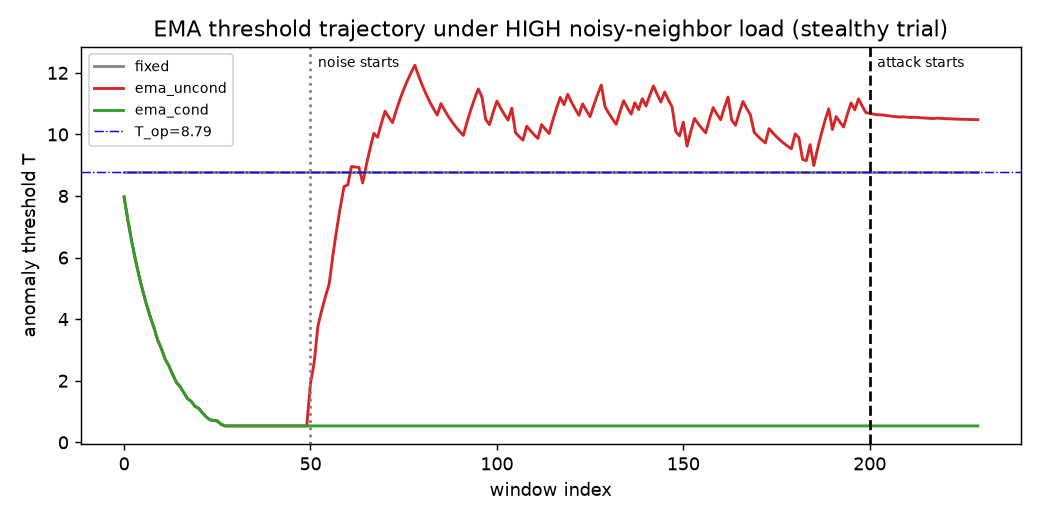
\includegraphics[width=0.92\textwidth]{figures/fig1_threshold.png}
\caption{Quỹ đạo ngưỡng $T$ trong một lượt thử nhiễu cao (tấn công stealthy). Khi nhiễu bắt đầu (cửa sổ 50), \texttt{ema\_uncond} (đỏ) bị kéo vọt lên \textit{trên} $T_{op}=8{,}79$ và duy trì ở mức cao suốt giai đoạn tấn công (từ cửa sổ 200) nên bỏ sót tấn công; \texttt{ema\_cond} (xanh) giảm về sàn $\approx0{,}5$ và giữ nguyên nên vẫn bắt được.}
\label{fig:traj}
\end{figure}

\begin{figure}[ht]
\centering
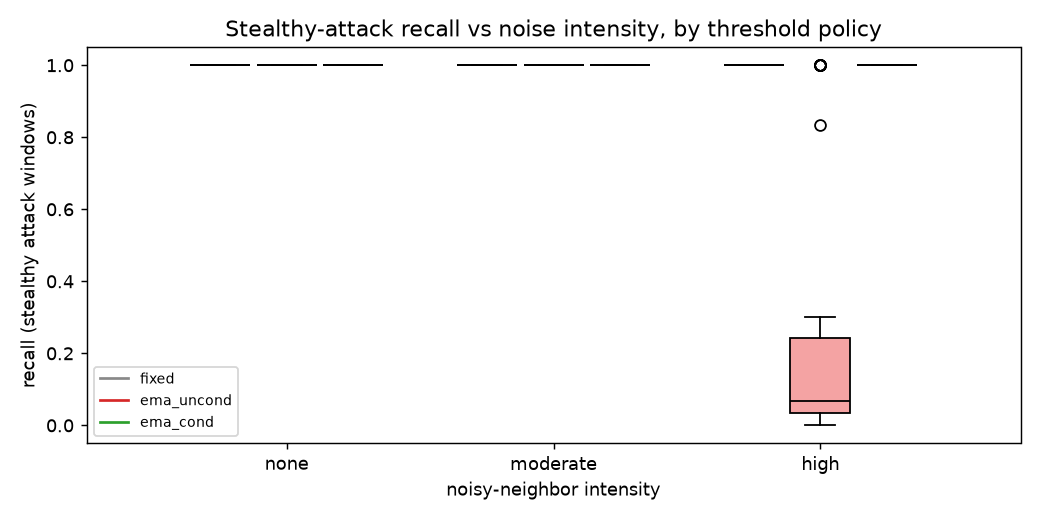
\includegraphics[width=0.92\textwidth]{figures/fig2_recall.png}
\caption{Recall của tấn công stealthy theo cường độ nhiễu, phân theo chính sách (box-plot trên 40 trial). Ở mức none/moderate cả ba chính sách đều đạt recall $1{,}0$; chỉ ở mức nhiễu cao, \texttt{ema\_uncond} (đỏ) sụt mạnh (trung vị $\approx0{,}06$), trong khi \texttt{fixed} và \texttt{ema\_cond} vẫn giữ $1{,}0$.}
\label{fig:recall}
\end{figure}
